\documentclass[11pt]{article}
\usepackage{mathtools}
\usepackage{mdframed}
\usepackage{fullpage}
\usepackage{amsfonts}
\usepackage{tikz}
\usepackage{fancyhdr}
\usepackage{lastpage}
\usetikzlibrary{automata, positioning}


%edit this for each class
\newcommand\name{John Collin Vincent}
\newcommand\classname{}
\newcommand\assignment{}


\newcounter{excounter}
\setcounter{excounter}{1}
\newcommand\ques[2]{\vskip 1em  \noindent\textbf{\arabic{excounter}\addtocounter{excounter}{1}.} \emph{#1} \noindent#2}
\newenvironment{question}{\ques{}\begin{quote}}{\end{quote}}


\pagestyle{fancy}
\rfoot{\name, page \thepage/\pageref{LastPage}}
\cfoot{}
\rhead{}
\lhead{}
\renewcommand{\headrulewidth}{0pt}
\renewcommand{\footrulewidth}{0pt}
\DeclarePairedDelimiter\ceil{\lceil}{\rceil}
\DeclarePairedDelimiter\floor{\lfloor}{\rfloor}


\begin{document}


  {\bf \classname \hspace{1cm} \assignment\hfill \name}
  \vskip 2em


  \begin{question}
    \begin{align*}
      S  &\rightarrow 1SZ | 0SE | \epsilon\\
      Z  &\rightarrow 0S\\
      E  &\rightarrow 1S
    \end{align*}\\
    for any string $w$ of 1's and 0's the CFG can copy the input fromm left to right, always
    keeping one S in the list of variables. While moving left to right any time $|1| > |0|$ the
    current state of the CFG will be $xSZ_1\ldots Z_k$ $x$ is the generate substring from
    the start of $w$ to the current posistion and $k = |x|_1 - |x|_0$.
    from there anytime a zero is the next character
    in $w$ the current $S$ can go to $\epsilon$ and the left most $Z$ can go to $0S$, reducing
    the number of $Z$'s in CFG by 1. The inverse is true for $|0| > |1|$. Using this parsing method
    anytime $|w|_0 = |w|_1$ the only variable in the CFG should be $S$ which can go to $\epsilon$
    accepting $w$ as a string in the language. Anytime $|w|_0 \ne |w|_1$ there will always be
    at lease one $Z$ or $E$ in the CFG after all the input is read causing the string to
    not be in the language.
  \end{question}

  \begin{question}
    \center
    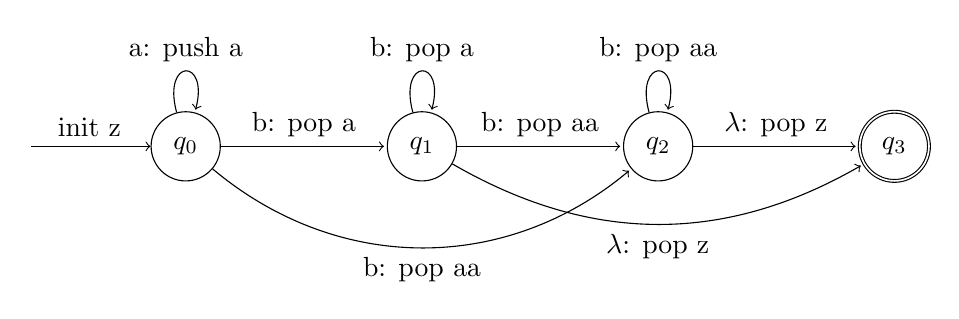
\begin{tikzpicture}[shorten >=1pt,node distance=3cm,on grid,auto]
      \node[state] (q_0) {$q_0$};
      \node[state] (q_1) [right=of q_0] {$q_1$};
      \node[state] (q_2) [right=of q_1] {$q_2$};
      \node[state, accepting] (q_3) [right=of q_2] {$q_3$};
      \draw[<-] (q_0) -- node[above] {init z} ++(-2cm, 0);
      \path[->]
      (q_0) edge [loop above] node [above] {a: push a} ()
            edge node [above] {b: pop a} (q_1)
            edge [bend right=40] node [below] {b: pop aa} (q_2);
      \path[->]
      (q_1) edge [loop above] node [above] {b: pop a} ()
            edge node [above] {b: pop aa} (q_2)
            edge [bend right=30] node [below] {$\lambda$: pop z} (q_3);
      \path[->]
      (q_2) edge [loop above] node [above] {b: pop aa} ()
            edge  node [above] {$\lambda$: pop z} (q_3);
    \end{tikzpicture}
  \end{question}

  \clearpage

  \begin{question}
    \center
    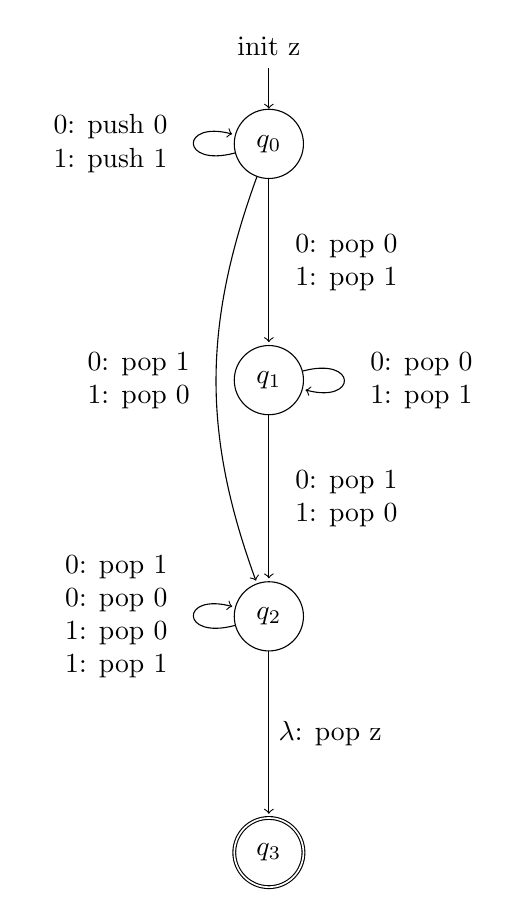
\begin{tikzpicture}[shorten >=1pt,node distance=3cm,on grid,auto]
      \node[state] (q_0) {$q_0$};
      \node[state] (q_1) [below=of q_0] {$q_1$};
      \node[state] (q_2) [below=of q_1] {$q_2$};
      \node[state, accepting] (q_3) [below=of q_2] {$q_3$};
      \draw[<-] (q_0) -- node [above, pos=1] {init z} ++(0, 1cm);
      \path[->]
      (q_0) edge [loop left] node [left] {
                                           \begin{tabular}{l}
                                             0: push 0\\
                                             1: push 1
                                           \end{tabular}
                                         } ()
            edge node [right] {
                                \begin{tabular}{l}
                                  0: pop 0\\
                                  1: pop 1
                                \end{tabular}
                              } (q_1)
            edge [bend right=20] node [left] {
                                               \begin{tabular}{l}
                                                 0: pop 1\\
                                                 1: pop 0
                                               \end{tabular}
                                             } (q_2);
      \path[->]
      (q_1) edge [loop right] node [right] {
        \begin{tabular}{l}
          0: pop 0\\
          1: pop 1
        \end{tabular}
      } ()
            edge node [right] {
              \begin{tabular}{l}
                0: pop 1\\
                1: pop 0
              \end{tabular}
            } (q_2);
      \path[->]
      (q_2) edge [loop left] node [left] {
        \begin{tabular}{l}
          0: pop 1\\
          0: pop 0\\
          1: pop 0\\
          1: pop 1
        \end{tabular}
      } ()
            edge node [right] {$\lambda$: pop z} (q_3);
    \end{tikzpicture}
  \end{question}


\end{document}
